\documentclass{article}
\usepackage[utf8]{inputenc}
\usepackage[top=80pt,bottom=80pt,left=88pt,right=86pt]{geometry}
\usepackage{amsthm}
\usepackage{amssymb}
\setcounter{tocdepth}{3}
\usepackage{graphicx}
\usepackage{algorithm}
\usepackage{microtype}
\usepackage{subfig}
\usepackage{amsmath}
\usepackage{amsthm}
\usepackage{enumerate}
\usepackage{wrapfig}
\usepackage{multirow}
\usepackage{nicefrac}
\usepackage[colorinlistoftodos,prependcaption,textsize=tiny]{todonotes}
\usepackage[colorlinks,linkcolor=blue,filecolor=blue,citecolor=blue,urlcolor=blue,pdfstartview=FitH,pagebackref]{hyperref}
\usepackage[nameinlink]{cleveref}
\usepackage{authblk}
\usepackage{algpseudocode}
\usepackage{amsmath}
\theoremstyle{remark}
\newtheorem*{remark}{Remark}
\bibliographystyle{plainurl}% the recommnded bibstyle

\usepackage{url}   
\newcommand{\keywords}[1]{\par\addvspace\baselineskip
	\noindent\keywordname\enspace\ignorespaces#1}

\usepackage{graphicx}
\graphicspath{ {./images/} }

\def\C{\mathcal{C}}
\def\G{\mathcal{G}}
\def\T{\mathcal{T}}
\def\I{\mathcal{I}}
\def\reals{{\mathbb R}}
\def\integers{{\mathbb Z}}
\def\natural{{\mathbb N}}
\def\eps{{\varepsilon}}
\def\diam{\rm diam}
\def\polylog{\rm polylog}

\DeclareMathOperator*{\argmax}{arg\,max}
\DeclareMathOperator*{\argmin}{arg\,min}

\newcommand{\opt}{\text{OPT}}
\newcommand{\vis}{\textit{Vis}}
\newcommand{\seg}[1]{\overline{#1}}
\newcommand{\uv}{\seg{uv}}
\newcommand{\xy}{\seg{xy}}
\newcommand{\xyp}{\seg{x'y'}}
\newcommand{\npc}{\textbf{NP}-complete}
\renewcommand{\arraystretch}{1.5}

\theoremstyle{definition}
\newtheorem{definition}{Definition}[section]

\newtheorem{observation}{Observation}[section]
\newtheorem{theorem}{Theorem}


\title{%
Dynamic time warping-based proximity problems}
\author{Matya, Boris}
\date{November 2019}

\begin{document}

\maketitle

\section{Background}

\paragraph{Dynamic Time Warping (DTW)}
Dynamic time warping (DTW) is a widely used curve similarity measure.
It was introduced~\cite{Keogh:2002:NTS:775047.775062} to
overcome the limitation of both global and local shifts.


DTW has been applied to temporal sequences of video, audio, and graphics data — indeed, any data that can be turned into a linear sequence can be analyzed with DTW. A well known application has been automatic speech recognition, to cope with different speaking speeds. Other applications include speaker recognition and online signature recognition. It can also be used in partial shape matching application\cite{wiki:Dynamic_time_warping}.

\subparagraph{Problem Formulation}
The dynamic time warping problem is stated as follows:


Given two curves:
\begin{center}
    $P=p_1, p_2,....p_{|P|}$, and $Q=q_1, q_2,....q_{|Q|}$
\end{center}
A path:
\begin{center}
    $W=w_1,w_2,....,w_{|W|}$, $w_k = (i, j)$
\end{center}
where $i$ is an index from $P$ and $j$ is an index from $Q$, every path has the following restrictions:

\begin{itemize}
    \item $w_1 = (1, 1)$ (each path starts from the first points in $P$ and $Q$)
    \item $w_{|W|} = (|P|, |Q|)$ (each path ends at the last points in $P$ and $Q$)
    \item $w_k = (i, j), w_{k+1} = (i',j')$ \qquad $i\leq i' \leq i+1$,  $j \leq j' \leq j+1$ (each item in the path either goes to the next point in $P$, the next point in $Q$ or both)
\end{itemize}
A path example:
\paragraph{}
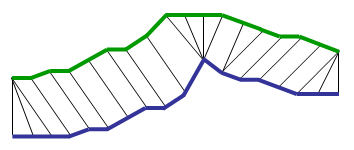
\includegraphics{aligned}
\paragraph{}

A distance of an item $w_k = (i, j)$ in a path is:
\begin{center}
    $Dist(w_k)=\lVert p_i q_j\rVert$ where $\lVert \cdot \rVert$ is the Euclidean norm
\end{center}

And a distance of a path is:
\begin{center}
    $Dist(W)=\sum_{k=1}^{|W|}{Dist(w_k)}$
\end{center}
$DTW(P,Q)$ is the path with $\min Dist(W)$ of all possible paths and $d_{DTW}(P, Q)$ is defined as $Dist(DTW(P,Q))$.
\paragraph{}
It is well-known that $d_{DTW}(P, Q)$ can be computed in $O(|P||Q|)$
time by a simple dynamic programming (DP) algorithm \cite{DBLP:journals/csr/Dietzfelbinger08}.

\section{Distance Oracle}
Our goal is to create an oracle that answers a 2-approximation DTW distance between a curve to a query segment
\begin{definition}
	Let C be a curve in d=1 with n points and let s = $\overline{pq}$ be a query segment. 
	Let the dynamic time warping(DTW) distance - $d_{dtw} (C, s)$. 
	
	Let $F(i)=\displaystyle\sum_{j=1}^{i}|C_j p|$,
	let $G(i)=\displaystyle\sum_{j=i+1}^{n}|C_j q|$ 
	and let $H(i)=F(i)+G(i)$
	
	So $D_{dtw}(C, s)=\displaystyle\min_{1\leq i\leq n-1}H(i)$
\end{definition}
\begin{observation}
	$F$ is an increasing function, 
	$G$ is a decreasing function and the functions intersect except for two cases: 1. $F$ is above $G$ for every $i$, in this case $i=1$ is minimal. 
	2. $G$ is above F for every $i$, in this case $i=n-1$ is minimal.
\end{observation}
\begin{theorem}
	Let k be the index before the intersection of $F$ and $G$
	
	Let $l=\argmin_{1\leq i\leq n-1}H(i)$
	
	We claim that $min(H(k), H(k+1))$ is a 2-approximation for $D_{dtw} (C, s)$ (or $H(l)$).
\end{theorem}
    \begin{proof}
    	Let's assume WLOG that $l\leq k$ so:
        $$2H(l)=2(F(l)+G(l))\geq 2G(l)\geq 2G(k)\geq F(k)+G(k)\geq H(k)$$
            
    	If $l>k$ we'll use $k+1$ instead of $k$ and replace $F$ with $G$
    \end{proof}
	Now our goal is to find $k$ in $O(\log^3n)$ and to get $H(k)$ using a $O(n\log n)$ storage.
	
	Implementation:
	If $F(1)>G(1)$ then the minimal value is $k=1$ else if $G(m)>F(m)$ then the minimal value is $k=n-1$ otherwise we'll perform a binary search that for each $i$ if $F(i)<G(i)$ then the next $i$ will be $i+\lfloor\dfrac{i}{2}\rfloor$ otherwise the next i will be $i-\lfloor\dfrac{i}{2}\rfloor$. In order to find $F(i)$ and $G(i)$ efficiently we are using orthogonal range tree that holds for each $C_i$ the point $(i, C_i)$ so the main tree holds the indices of points and each node maps to a tree that holds the values of points in the range of indices of that node, 
	and for each subtree in the values tree we'll hold at its root the number of points and their sum.
	
	Now since: 
	$$F(i)=\displaystyle\sum_{j=1}^{i}|C_j p| = \displaystyle\sum_{\substack{j=1 \\ C_j<p}}^{i}(p - C_j) + \displaystyle\sum_{\substack{j=1 \\ C_j>p}}^{i}(C_j - p)$$ 
	let's say that there are k points that $C_j<p$ and $j<i$ so:
	$$\displaystyle\sum_{\substack{j=1 \\ C_j<p}}^{i}(p - C_j) + \displaystyle\sum_{\substack{j=1 \\ C_j>p}}^{i}(C_j - p) =
	   k*p - \displaystyle\sum_{\substack{j=1 \\ C_j<p}}^{i}C_j - (i-k)*p +  \displaystyle\sum_{\substack{j=1 \\ C_j>p}}^{i}C_j$$
	   
	Now to compute $F(i)$ and $G(i)$ we'll use the following simple algorithms:

\begin{algorithmic}
  \Procedure{$F$}{$i$}\Comment{$T$ is the orthogonal range tree, $i$ is the index and $p$ is the point from the segment}
  	\State $res\gets |p, C_i|$
  	\State $Q_1\gets T(indices<i, values<p)$
  	\State $res\gets res +  p*\displaystyle\sum_{r\in Q_1}{count(r)} - \displaystyle\sum_{r\in Q_1}{sum(r)}$
  	\State $Q_2\gets T(indices<i, values>p)$
 	\State $res\gets res + p*\displaystyle\sum_{r\in Q_2}{sum(r)}  - p*\displaystyle\sum_{r\in Q_2}{count(r)}$
 	\State \textbf{return} $res$
  \EndProcedure
\end{algorithmic}
\begin{algorithmic}
	\Procedure{$G$}{$i$}\Comment{$T$ is the orthogonal range tree, $i$ is the index and $q$ is the point from the segment}
	\State $res\gets |q, C_i|$
	\State $Q_1\gets T(indices>i, values<q)$
	\State $res\gets res + count(Q_1)*q - sum(Q_1)$
	\State $Q_2\gets T(indices>i, values>q)$
	\State $res\gets res + sum(Q_2) - count(Q_2)*q$
	\State \textbf{return} $res$
	\EndProcedure
\end{algorithmic}
%\begin{observation}
%	The queries that we perform on the main tree in our orthogonal range tree are only $x>i$ or 
%	$x<i$ that means 2(m-1) possible queries so we can store the results(values trees) in 2 (m-1)-size arrays
% instead of the main(indices) tree so we'll get query time - $O(log^2n)$ instead of $O(log^3n)$ with the same storage.
%\end{observation}
\begin{theorem}
	Same algorithm can be applied for d dimensions in $L_1$ metric in $O(d\log ^3n)$ and to using a $O(d*n\log n)$ storage.
\end{theorem}
\begin{proof}
	We'll demonstrate for $d=2$ and the same logic can be applied for d dimensions.
	The binary search stays the same, the only thing that changes is the way we compute $F(i)$ and $G(i)$:
$$F(i)=\displaystyle\sum_{j=1}^{i}|C_j p| = \displaystyle\sum_{j=1}^{i}|C^x_j - p^x| + \displaystyle\sum_{j=1}^{i}|C^y_j - p^y|$$
	 
	 Now we can compute each component the same way we computed in $d=2$ so we'll double the time and storage complexity.
\end{proof}
\begin{observation}
	Our oracle supports also dynamic setting where you can insert, delete and update points in the curve.
	Since we hold $O(d*n)$ trees and insert, delete and update on each tree is $O(\log n)$ and creating a new tree is $O(n\log n)$ so the total of every action is $O(d*n\log n)$.
\end{observation}


\section{Curve Center}
Let $\mathcal{C}  = \{C_1,\ldots,C_n\}$ be a set of $n$ $m$-curves and let $K$ be a small positive integer. We consider the ``curve center'' problem for ${\cal C}$, i.e., find a curve $c'$ of length $K$ for which $$\max \{d_{DTW}(c',C_1),\ldots,d_{DTW}(c',C_n)\}$$ is minimum. We wish to construct an algorithm that finds the curve center or an approximation to it.
\paragraph{}
Solving for $K=2$ for $L_\infty$ norm:
Let's first solve for $d=1$, let's define $\tau=(\tau_1,\ldots, \tau_{(m-1)(n-1)})$ such that $\tau_i$ represents the segment between 2 adjacent points (after sorting) $l(tau_i), r(tau_i)\in C=C_1\bigcup \ldots \bigcup C_n$.

\subsection{Linear program solution}
For each possible pair of $(\tau_a, \tau_b)$ we'll define a linear program for finding the best segment $(a, b)$ in this $\tau$ after running all possible $O(n^2 M^2)$ programs we'll find the minimum of all programs and return it.

Let's define the linear program for $(\tau_a, \tau_b)$:
\begin{equation*}
\begin{array}{ll@{}ll}
\text{minimize}  & z\\
\text{subject to}&
l(\tau_a) \leq a \leq r(\tau_a) \\
&l(\tau_b) \leq b \leq r(\tau_b) \\
&F_1 \leq 
\displaystyle\sum\limits_{\substack{p_i \in C_1\\ i\leq j \\ p_i \leq l(\tau_a)}}{(a - p_i)} +   
\displaystyle\sum\limits_{\substack{p_i \in C_1\\ i\leq j \\ p_i \geq r(\tau_a)}}{(p_i - a)} +   
\displaystyle\sum\limits_{\substack{p_i \in C_1\\ i>j     \\ p_i \leq l(\tau_b)}}{(b - p_i)} +   
\displaystyle\sum\limits_{\substack{p_i \in C_1\\ i>j     \\ p_i \geq r(\tau_b)}}{(p_i - b)}   
&&j=1,...,m-1\\

&\vdots\\
&F_n \leq 
\displaystyle\sum\limits_{\substack{p_i \in C_n\\ i\leq j \\ p_i \leq l(\tau_a)}}{(a - p_i)} +   
\displaystyle\sum\limits_{\substack{p_i \in C_n\\ i\leq j \\ p_i \geq r(\tau_a)}}{(p_i - a)} +   
\displaystyle\sum\limits_{\substack{p_i \in C_n\\ i>j     \\ p_i \leq l(\tau_b)}}{(b - p_i)} +   
\displaystyle\sum\limits_{\substack{p_i \in C_n\\ i>j     \\ p_i \geq r(\tau_b)}}{(p_i - b)}   
&&j=1,\ldots,m-1\\
%x_{j} \in \{0,1\}, &j=1 ,..., m
&z \geq F_i &&i=1,\ldots,n
\end{array}
\end{equation*}


\subsection{A more efficient solutions}

\subsubsection{First solution}
For every possible pair of $(\tau_a, \tau_b)$ we'll define for every curve $C_i$ and for every $j\in1,\ldots,m$ we'll create a bivariate function:
$$f(a, b) = \displaystyle\sum\limits_{\substack{p_i \in C_i\\ i\leq j \\ p_i \leq l(\tau_a)}}{(a - p_i)} +   
\displaystyle\sum\limits_{\substack{p_i \in C_i\\ i\leq j \\ p_i \geq r(\tau_a)}}{(p_i - a)} +   
\displaystyle\sum\limits_{\substack{p_i \in C_i\\ i>j     \\ p_i \leq l(\tau_b)}}{(b - p_i)} +   
\displaystyle\sum\limits_{\substack{p_i \in C_i\\ i>j     \\ p_i \geq r(\tau_b)}}{(p_i - b)}$$

\paragraph{}
\label{firstsolotion}
So for each curve $C_i$ we have $m$ functions, let $S(C_i)$ denote the LOWER envelope of those functions. So we have $n$ convex surfaces $S_1, \ldots, S_n$ each of complexity $O(m)$ and $O(n m)$ facets in total that we can assume are triangulated, it's an UPPER envelope $U$ of $K=O(n m)$ triangles and therefore has the complexity $O(K^2\alpha(K))=O(n^2 m^2\alpha(n m))$ \cite{DBLP:journals/dcg/EdelsbrunnerGS89} \cite{DBLP:journals/dcg/PachS89}, let $V_{\tau_a, \tau_b}$ denote the minimum vertex of this envelope, we will return the $\min V_{\tau_a, \tau_b}$ over all $\tau$'s, since there are $O(n^2 m^2)$
possible $\tau$'s the total complexity is $O(n^4 m^4\alpha(n m))$.

This solutions can be extended to higher dimensions in $L_\infty$, all we have to do is redefine our $\tau$'s according to $L_\infty$ so we get $O((n m)^d)$ $\tau$'s and $O((n m)^{2d})$ pairs of $\tau$'s so we get total complexity $O((n m)^{2d + 2}\alpha(n m))$
\paragraph{}

\subsubsection{Second solution}
Another approach is for each curve $C_i$ to split the curve to $m+1$ $\tau$'s according to $C_i$ points sorted by their $x$-coordinate, for each rectangle $(\tau_a, \tau_b)$ in the $x-y-$-plane of $C_i$ take the LOWER envelope of all possible partitions in this rectangle, since every function in this rectangle is linear, the LOWER envelope's complexity is $O(m)$ and there are $O(m^2)$ rectangles for total function $O(m^3)$ facets, so we have a piecewise-linear function of complexity $O(m^3)$ for each curve $C_i$ for a total of $K=O(n m^3)$ facets, the UPPER envelope of those $n$ functions is of complexity $O(K^2\alpha(K))=O(n^2 m^6\alpha(n m^3)))$ and pick its lowest point as our result.

This solutions can also be extended to higher dimensions in $L_\infty$, all we have to do is redefine our $\tau$'s according to $L_\infty$ so we get $O(m^d)$ $\tau$'s for every curve and $O(m^{2d})$ pairs of $\tau$'s so we get total complexity $O(m^{4d + 2} n \alpha(n m^{2d + 1}))$

% Another approach is to find first the lower envelope of the functions of each curve, for each curve this $\tau_a, \tau_b$, each lower envelope has $O(m)$ complexity and there are $O(m^2)$ (or $O(m^2n^2)$ ??) for a total $O(m^2)$ (or $O(m^2n^2)$
% let $S_{a,b}$ represent this lower envelope, now we'll find the upper envelope of all possible $S_{a,b}$ and return the minimum value of it.

\section{Nearest neighbour(NN)}
Let $\mathcal{C} = \{C_1,\ldots,C_n\}$ be a set of $n$ $m$-curves positive, we preprocess $\mathcal{C}$ and create $O((n m)^{2d})$ envelopes as defined in the \hyperref[firstsolotion]{first solution} of segment center but instead of UPPER envelopes we will take the LOWER envelope, for each envelope we will store create a segment tree, so when for each query segment $(p,q)$ we first find the $\tau$'s containing $p$ and $q$ in $O(\log^{d} ((n m)^{d})))$ and then we find the curve in the segment tree in $O(\log^{d+2} ((n m)^{2d}))$.

\bibliography{refs}

\end{document}
